%-----------------------------------------------------------------------------
%
%               Template for sigplanconf LaTeX Class
%
% Name:         sigplanconf-template.tex
%
% Purpose:      A template for sigplanconf.cls, which is a LaTeX 2e class
%               file for SIGPLAN conference proceedings.
%
% Guide:        Refer to "Author's Guide to the ACM SIGPLAN Class,"
%               sigplanconf-guide.pdf
%
% Author:       Paul C. Anagnostopoulos
%               Windfall Software
%               978 371-2316
%               paul@windfall.com
%
% Created:      15 February 2005
%
%-----------------------------------------------------------------------------


%\documentclass[preprint]{sigplanconf}
\documentclass[10pt]{sigplanconf}

% The following \documentclass options may be useful:
%
% 10pt          To set in 10-point type instead of 9-point.
% 11pt          To set in 11-point type instead of 9-point.
% authoryear    To obtain author/year citation style instead of numeric.

\usepackage{yfonts}
\usepackage{amsmath}
\usepackage{amssymb}
\usepackage{mathpartir}
\usepackage{url}
\usepackage{graphics}
\usepackage{graphicx}
\usepackage{marvosym}
\usepackage{stmaryrd}
\usepackage{epsdice}
\usepackage[usenames,dvipsnames]{xcolor}
\usepackage[utopia]{mathdesign}

% ____________________________________________________________
% Listings Package Configuration
% \usepackage[scaled]{beramono}

\renewcommand*\ttdefault{txtt}
\usepackage[T1]{fontenc}

\RequirePackage{listings}
% \lstdefinelanguage{Rust}{
%   morekeywords={fn,let,enum,if,else,return,mut,const,copy,ref,move,match,struct,type,int,while,float,as,fail},
%   sensitive=true,
%   morecomment=[l]{//},
%   morecomment=[s]{/*}{*/},
%   morestring=[b]",
% }
% \lstset{language=Rust,
%         frame=none,%single,
%         basicstyle=\ttfamily\footnotesize,
%         keywordstyle=\bfseries,
%         commentstyle=\footnotesize,
%         tabsize=2,
%         showstringspaces=false,
%         flexiblecolumns=false,
%         mathescape=true,
%         escapeinside={\#}{\#},
%         % numbers=left, numberstyle=\tiny, numbersep=5pt %, stepnumber=2, 
%         % literate={->}{{$\rightarrow$}}1 {<->}{{$\leftarrow$}}1
% }

% This Deep Tex Voodoo is from
%   <http://www.latex-community.org/forum/viewtopic.php?f=5&t=2072>
% It's purpose is to make \lstinline normal size, without affecting
% \lstinputlisting.  It seems to work but I have no idea how or why,
% and I rather hope never to learn.
\makeatletter
\lst@AddToHook{TextStyle}{\let\lst@basicstyle\ttfamily\normalsize}
\makeatother

\newcommand{\Figref}[1]{Figure \ref{#1}}
\newcommand{\Secref}[1]{Section \ref{#1}}
\newcommand{\x}[1]{\lstinline{#1}}

% ______________________________________________________________________
% Formatting commands for terminals, non-terminals, and so forth

\newcommand{\TypeRulesSize}{\normalsize}
\newcommand{\TypeRules}[1]{\begin{mathpar} \TypeRulesSize #1 \end{mathpar}}

\newcommand{\terminal}[1]{\ensuremath{\text{\emph{#1}}}}
\newcommand{\nonterminal}[1]{\ensuremath{\text{\emph{#1}}}}
\newcommand{\keyword}[1]{\ensuremath{\textsf{#1}}}
\newcommand{\rep}[1]{\ensuremath{\overline{#1}}}
\newcommand{\tyfunction}[1]{\ensuremath{\textsc{#1}}}

\newcommand{\Env}{\ensuremath{\Gamma}}
\newcommand{\Subtype}{\ensuremath{\mathtt{<:}}}
\newcommand{\Lt}{\ensuremath{\mathtt{<}}}
\newcommand{\Gt}{\ensuremath{\mathtt{>}}}

\newcommand{\Lb}{\keyword{\{}}
\newcommand{\Rb}{\keyword{\}}}

\newcommand{\Pipe}{\ensuremath{\quad|\quad}}

\newcommand{\Zero}{\ensuremath{\textsf{Z}}}
\newcommand{\Suc}[1]{\ensuremath{\textsf{S(}#1\textsf{)}}}
\newcommand{\Let}[3]{\ensuremath{\textcolor{Black}{\textsf{let~}}#1\textcolor{Black}{\textsf{~=~}}#2\textcolor{Black}{\textsf{~in~}}#3}}
\newcommand{\Case}[4]{\ensuremath{\textsf{case~}#1\textsf{~of~}\Zero~\Rightarrow~#2;~\Suc{#3}~\Rightarrow~#4}}

\newcommand{\Grammar}{
  \begin{tabular}{llll}
    $e$ & = & $\lambda x. e$ \Pipe $e_1 e_2$ & {\em functions} \\
    & | & $x[\rep{e}]$ & {\em random variables} \\
    & | & \Zero \Pipe \Suc{e} & {\em natural numbers} \\
    & | & \Case{e_1}{e_2}{x}{e_3} & {\em natural induction} \\
    & | & \Let{x}{e_1}{e_2} & {\em eager evaluation}
  \end{tabular}
}

\newcommand{\Val}{\textcolor{Cerulean}{\textsf{val}}}
\newcommand{\subst}[2]{\textcolor{OliveGreen}{\llparenthesis #1} \textcolor{OliveGreen}{/ #2} \textcolor{OliveGreen}{\rrparenthesis}}
\newcommand{\substeq}{=}
\newcommand{\capture}[2]{\textcolor{RedOrange}{\leftwave #1 / #2 \rightevaw}}
\newcommand{\captureeq}{=}
\newcommand{\eval}{\textcolor{WildStrawberry}{~\ensuremath{\mapsto}~}}
\newcommand{\evalstar}{\textcolor{WildStrawberry}{~\ensuremath{\mapsto^*}~}}

% Evaluation

\newcommand{\EvalVar}{
	\inferrule[Eval-Var]{
	}{
		x[\rep{e}]~\Val
	}
}
\newcommand{\EvalLam}{
	\inferrule[Eval-Lam]{
	}{
		\lambda x.e~\Val
	}
}
\newcommand{\EvalApp}{
	\inferrule[Eval-App]{
		e_1 \eval \lambda x. e_1'
	}{
		e_1 e_2 \eval \subst{e_2}{x}e_1'
	}
}
\newcommand{\EvalZero}{
	\inferrule[Eval-Zero]{
	}{
		\Zero~\Val
	}
}
\newcommand{\EvalSucA}{
	\inferrule[Eval-Suc-1]{
		e~\Val
	}{
		\Suc{e}~\Val
	}
}
\newcommand{\EvalSucB}{
	\inferrule[Eval-Suc-2]{
		e \eval e'
	}{
		\Suc{e}\eval\Suc{e'}
	}
}
\newcommand{\EvalCaseA}{
	\inferrule[Eval-Case-1]{
		e_1 \eval \Zero
	}{
		\Case{e_1}{e_2}{x}{e_3} \eval e_2
	}
}
\newcommand{\EvalCaseB}{
	\inferrule[Eval-Case-2]{
		e_1 \evalstar \Suc{n} \quad \Suc{n}~\Val
	}{
		\Case{e_1}{e_2}{x}{e_3} \eval \subst{n}{x}e_3
	}
}
\newcommand{\EvalLet}{
	\inferrule[Eval-Let]{
		e_1 \evalstar e_1' \quad e_1'~\Val
	}{
		\Let{x}{e_1}{e_2} \eval \subst{e_1'}{x}e_2
	}
}

% Substitution

\newcommand{\SubstLam}{
	\inferrule[Subst-Lam]{
		y \ne x
	}{
		\subst{e_0}{x} \lambda y.e \substeq \lambda y.\subst{e_0}{x}e'
	}
}
\newcommand{\SubstCapture}{
	\inferrule[Subst-Capture]{
	}{
		\subst{e_0}{x} \lambda x.e \substeq \lambda x.\capture{e_0}{x}e
	}
}
\newcommand{\SubstLamCapture}{
	\inferrule[Subst-Lam-Capture]{
	}{
		\subst{e_0}{x} \lambda x.e \substeq \lambda x.\capture{e_0}{x}e
	}
}
\newcommand{\SubstApp}{
	\inferrule[Subst-App]{
	}{
		\subst{e_0}{x} e_1 e_2 \substeq \subst{e_0}{x}e_1 \subst{e_0}{x} e_2'
	}
}
\newcommand{\SubstVarY}{
	\inferrule[Subst-Var-Y]{
		y \ne x \quad
	}{
		\subst{e_0}{x} y[\rep{e}] \substeq y[\subst{e_0}{x}\rep{e}]
	}
}
\newcommand{\SubstVarX}{
	\inferrule[Subst-Var-X]{
		e_1 \in \left ( e_0,\subst{e_0}{x}\rep{e} \right )
	}{
		\subst{e_0}{x} x[\rep{e}] \substeq e_1
	}
}
\newcommand{\SubstZero}{
	\inferrule[Subst-Zero]{
	}{
		\subst{e_0}{x} \Zero \substeq \Zero
	}
}
\newcommand{\SubstSuc}{
	\inferrule[Subst-Suc]{
	}{
		\subst{e_0}{x} \Suc{e} \substeq \Suc{\subst{e_0}{x}e}
	}
}
\newcommand{\SubstCaseCapture}{
	\inferrule[Subst-Case-Capture]{
	}{
		\subst{e_0}{x} \Case{e_1}{e_2}{x}{e_3} \substeq \Case{\subst{e_0}{x}e_1}{\subst{e_0}{x}e_2}{x}{\capture{e_0}{x}e_3}
	}
}
\newcommand{\SubstCase}{
	\inferrule[Subst-Case]{
		y \ne x
	}{
		\subst{e_0}{x} \Case{e_1}{e_2}{y}{e_3} \substeq \Case{\subst{e_0}{x}e_1}{\subst{e_0}{x}e_2}{y}{\subst{e_0}{x}e_3}
	}
}
\newcommand{\SubstLetCapture}{
	\inferrule[Subst-Let-Capture]{
	}{
		\subst{e_0}{x} \Let{x}{e_1}{e_2} \substeq \Let{x}{\subst{e_0}{x}e_1}{\capture{e_0}{x}e_2}
	}
}
\newcommand{\SubstLet}{
	\inferrule[Subst-Let]{
		y \ne x
	}{
		\subst{e_0}{x} \Let{y}{e_1}{e_2} \substeq \Let{y}{\subst{e_0}{x}e_1}{\subst{e_0}{x}e_2}
	}
}

% Capture

\newcommand{\CaptureLam}{
	\inferrule[Capture-Lam]{
	}{
		\capture{e_0}{x} \lambda y.e \captureeq \lambda y.\capture{e_0}{x}e'
	}
}
\newcommand{\CaptureApp}{
	\inferrule[Capture-App]{
	}{
		\capture{e_0}{x} e_1 e_2 \captureeq \capture{e_0}{x}e_1 \capture{e_0}{x} e_2'
	}
}
\newcommand{\CaptureVarY}{
	\inferrule[Capture-Var-Y]{
		y \ne x \quad
	}{
		\capture{e_0}{x} y[\rep{e}] \captureeq y[\capture{e_0}{x}\rep{e}]
	}
}
\newcommand{\CaptureVarX}{
	\inferrule[Capture-Var-X]{
	}{
		\capture{e_0}{x} x[\rep{e}] \captureeq x[e_0,\capture{e_0}{x}\rep{e}]
	}
}
\newcommand{\CaptureZero}{
	\inferrule[Capture-Zero]{
	}{
		\capture{e_0}{x} \Zero \captureeq \Zero
	}
}
\newcommand{\CaptureSuc}{
	\inferrule[Capture-Suc]{
	}{
		\capture{e_0}{x} \Suc{e} \captureeq \Suc{\capture{e_0}{x}e}
	}
}
\newcommand{\CaptureCase}{
	\inferrule[Capture-Case]{
	}{
		\capture{e_0}{x} \Case{e_1}{e_2}{y}{e_3} \captureeq \Case{\capture{e_0}{x}e_1}{\capture{e_0}{x}e_2}{y}{\capture{e_0}{x}e_3}
	}
}
\newcommand{\CaptureLet}{
	\inferrule[Capture-Let]{
	}{
		\capture{e_0}{x} \Let{y}{e_1}{e_2} \captureeq \Let{y}{\capture{e_0}{x}e_1}{\capture{e_0}{x}e_2}
	}
}

\begin{document}

\conferenceinfo{SIGBOVIK '13}{Pittsburgh, PA, USA}
\copyrightyear{2013}
\copyrightdata{}

\titlebanner{banner above paper title}        % These are ignored unless
\preprintfooter{short description of paper}   % 'preprint' option specified.

\title{
% Random Scope for Syntactic Hope
% Learning to Cope with Random Scope
Randomly-Scoped Lambda Calculus
}
% \subtitle{\em The Randomly-Scoped Lambda Calculus}
% \subtitle{Subtitle Text, if any}

\authorinfo{Ben Blum}{}{bblum@cs.cmu.edu}

%\authorinfo{
%  Nicholas D. Matsakis
%  \and Brian Anderson
%  \and Ben Blum \\
%  \and Tim Chevalier 
%  \and Graydon Hoare
%  \and Patrick Walton
%  \and David Herman}
%           {Mozilla Research}
%           {\{nmatsakis, banderson\}@mozilla.com,
%             bblum@cs.cmu.edu, \\
%             \{tchevalier, graydon, pwalton, dherman\}@mozilla.com}

\maketitle

\begin{abstract}

Gaze upon the following travesty, which Python hath wrought upon the world:
\begin{verbatim}
    >>> x
    NameError: name 'x' is not defined
    >>> [x for x in 1,2,3]
    [1, 2, 3]
    >>> x
    3
    >>>
\end{verbatim}

The question of {\em scope} pertains to the set of rules governing which values a program's variables refer to during evaluation.
Prior work has proposed two main approaches: {\em static} (or {\em lexical}) {\em scope}, in which variable bindings are resolved through source code analysis, and {\em dynamic scope}, in which bindings are resolved at run-time using a stack of activation records.

In this work, I present {\em random scope}, a new technique for scoping, as an alternative to the above two.
Random scope affords programmers the flexibility to refer to multiple different binding sites simultaneously; for example, applying the term $(\lambda x. (\lambda x. x))$ to two arguments could evaluate to either the first or the second one.
I figure out what kind of evaluation semantics would make this work, and then pretty much stumble onwards from there trying to make sense of the whole damn thing.

I define the Randomly-Scoped Lambda Calculus, and show how it can be used to compute random natural numbers, while also providing more popular deterministic functionalities such as factorial and fibonacci.

\end{abstract}

% \category{D.3.3}{Language Constructs and Features}{Data types and structures}

\keywords
static scope, dynamic scope, lower is better

\section{Introduction}

Some modern programming languages~\cite{wikiplia,python,lambda,sml,GoLang,RustLang,mla,haskell98,patenttroll} include a mechanism to refer to previously-computed values using more consise names, typically called {\em variables}. The question then arises: ``Which values should my variables refer to?''
In a half-hearted attempt to answer, these languages implement {\em scope} (which I explained in the abstract; go read it), and hope it all works out okay.

Whether resolved statically or dynamically, modern scoping approaches lack the flexibility to refer to multiple binding sites simultaneously.
I present the Randomly-Scoped Lambda Calculus (RSLC), in which references to shadowed variables can evaluate to any of their binding sites with equal probability.

Consider the following lambda calculus term:
\[ (\lambda x. (\lambda x. x))~A~B \]
In ordinary lambda calculus, this always evaluates to $B$ (quite unforgivingly so, in my opinion).
However, I give the programmer the benefit of the doubt, and assume they named the first argument $x$ as well because they wanted it to have equal opportunity. Hence, in RSLC this term can evaluate to either $A$ or $B$.
(On the other side of the coin, RSLC encourages good programming practice: a programmer who {\em doesn't} want $x$ to evaluate to $A$ should name the first argument something different, to make their intentions more clear.)

In this paper I make the following contributions:
\begin{enumerate}
	\item The {\bf Randomly-Scoped Lambda Calculus (RSLC)}, a logical programming language that uses a novel syntactic technique called {\bf random scoping},
	%\item An analysis of two implementation strategies for random scoping, which I call {\bf static random scope (SRS)} and {\bf dynamic random scope (DRS)},
	\item A new schema for general recursion in RSLC (because the Y combinator doesn't work anymore),
	\item Programming examples in RSLC that employ random scope to compute random natural numbers,
	\item Programming examples in RSLC that avoid random scope to implement deterministic arithmetic.
\end{enumerate}

\section{Language Definition}

\begin{figure}[t]
	\Grammar
	\caption{RSLC formal grammar.}
	\label{fig:grammar}
\end{figure}

RSLC is an extention to the lazy un(i)typed lambda calculus with slightly modified substitution rules. In the grammar (Figure~\ref{fig:grammar}), a variable $x$ carries around a list of expressions $\rep{e}$ which we have ``tried to substitute for it before''.
When programming in RSLC, we simply write $x$ (or $y$ or \Neptune~or however you happen to swing), because no substitution has happened yet, but after $n$ ``$\lambda x$''s have been $\beta$-reduced, the $\rep{e}$ list will have $n$ expressions in it.
It might help to think of it like quantum superposition, I guess?

Anyway, Figure~\ref{fig:eval} shows the evaluation rules, which are basically what you'd expect, and Figure~\ref{fig:subst} shows the substitution rules, which are new.
In the normal $\lambda$-calculus, substitution would stop when a new binding's name is the same as the one being substituted for.

However, in RSLC, as shown in {\sc Subst-Lam-Capture}, we switch to a second substitution mode, {\sc Capture}, in which substituted expressions are appended to a variable's $\rep{e}$ list (in the {\sc Capture-Var-X} rule).
Similarly, when substituting for $x$ before switching to {\sc Capture} mode (in the {\sc Subst-Var-X} rule), we nondeterministically select an expression from $x$'s $\rep{e}$ list to replace $x$ with (with uniform randomness).

\begin{figure}[t]
	\fbox{\begin{tabular}{ll}$e \eval e'$ \\ $e~\Val$\end{tabular}}
	\TypeRules{
		\EvalLam \qquad \EvalApp \qquad \EvalVar \\
		\EvalZero \qquad \EvalSucA \qquad \EvalSucB \\
		\EvalCaseA \\ \EvalCaseB \\ \EvalLet
	}
	\caption{RSLC small-step evaluation rules. They're exactly the same as for any other call-by-name $\lambda$-calculus, so don't bother reading them. Why am I even including them?}
	\label{fig:eval}
\end{figure}

\begin{figure}[t]
	\fbox{$\subst{e_0}{x}{e}$}
	\TypeRules{
		\SubstLamCapture \qquad \SubstLam \\
		\SubstVarX \qquad \SubstVarY \\
	}
	\fbox{$\capture{e_0}{x}{e}$}
	\TypeRules{
		\CaptureVarX \qquad \CaptureVarY \\
	}
	\caption{RSLC substitution rules. The ``$e_1 \in ...$'' premise in {\sc Subst-Var-X} represents nondeterministic choice. (Only important rules are shown here; Figure~\ref{fig:subst-complete} shows the complete set.)}
	\label{fig:subst}
\end{figure}

\subsection{Evaluation Example} 

As an example, I present the steps for evaluating the $(\lambda x. (\lambda x. x))~A~B$ from the introduction:

\begin{eqnarray*}
	& & (\lambda x. (\lambda x. x[]))~A~B \\
	& \mapsto & (\subst{A}{x} (\lambda x. x[])) B \\
	& = & (\lambda x. \capture{A}{x} x[]) B \\
	& = & (\lambda x. x[A]) B \\
	& \mapsto & \subst{B}{x} x[A] \\
	& = & \text{\em (any element of the list $[B,A]$)}
\end{eqnarray*}

\section{Random Programming with RSLC}

Already we have a system with which we can implement simple random number generators, such as a simple 6-sided die:
\[
(\lambda x.
(\lambda x.
(\lambda x.
(\lambda x.
(\lambda x.
(\lambda x. x))))))
~\epsdice{1}
~\epsdice{2}
~\epsdice{3}
~\epsdice{4}
~\epsdice{5}
~\epsdice{6}
\]

However, 

\newpage

\section{Evaluation}

We computed some random numbers woo

\begin{figure}[t]
	\begin{center}
	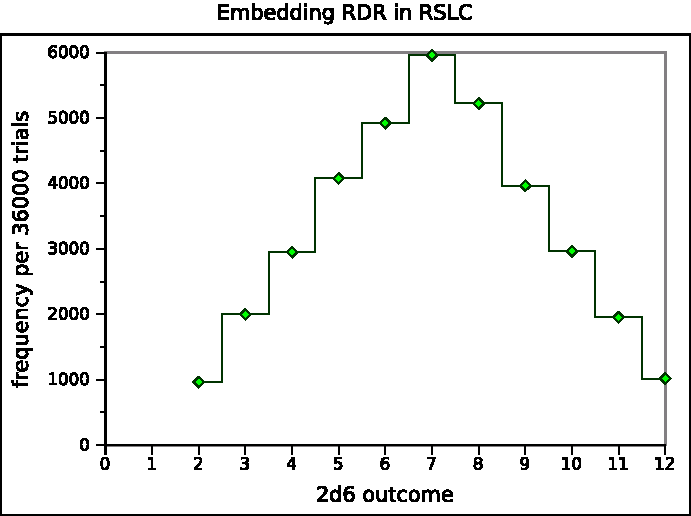
\includegraphics[width=0.48\textwidth]{rslc-rdr.pdf}
	\end{center}
	\caption{We show that RSLC is a generalization of the Random Distance Run~\cite{rdr}.}
	\label{fig:rdr}
\end{figure}

\begin{figure}[t]
	\begin{center}
	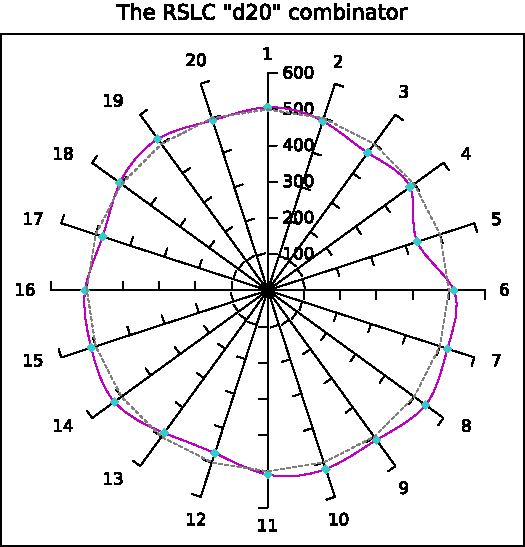
\includegraphics[width=0.40\textwidth]{rslc-d20.pdf}
	\end{center}
	\caption{RSLC can also be used to implement popular role-playing games.}
	\label{fig:rdr}
\end{figure}

\bibliographystyle{alpha}
\bibliography{paper}

\appendix

\section{Discussion of Substitution Rules}
\begin{figure*}[t]
	\fbox{$\subst{e_0}{x}{e}$}
	\TypeRules{
		\SubstLamCapture \qquad \SubstLam \qquad
		\SubstApp \\
		\SubstVarX \qquad \SubstVarY \\
		\SubstCaseCapture \\ \SubstCase \\
		\SubstZero \qquad \SubstSuc \\
		\SubstLetCapture \qquad \SubstLet
	}
	\fbox{$\capture{e_0}{x}{e}$}
	\TypeRules{
		\CaptureLam \qquad \CaptureApp \qquad
		\CaptureVarX \qquad \CaptureVarY \\
		\CaptureCase \\
		\CaptureZero \qquad \CaptureSuc \qquad \CaptureLet
	}
	\caption{Complete RSLC substitution and capture rules.}
	\label{fig:subst-complete}
\end{figure*}

\end{document}
